% Compile with XeLaTeX, TeXLive 2013 or more recent
\documentclass{beamer}

% Base packages
\usepackage{fontspec}
\usepackage{xunicode}
\usepackage{xltxtra}

\usepackage{amsfonts}
\usepackage{amsmath}
\usepackage{longtable}
\usepackage{csquotes}
\usepackage{standalone}

% Setup fonts
\newfontfamily\russianfont{CMU Serif}
\setromanfont{CMU Serif}
\setsansfont{CMU Sans Serif}
\setmonofont{CMU Typewriter Text}

% Setup Russian hyphenation. NOTE: this declaration *must* come after fontspec's font declarations,
% or a mysterious (but harmless in other respects) error "Improper `at' size (0.0pt), replaced by 10pt." would appear.
\usepackage{polyglossia}
\defaultfontfeatures{Scale=MatchLowercase, Mapping=tex-text}

\setdefaultlanguage[spelling=modern]{russian} % for polyglossia
\setotherlanguage{english} % for polyglossia

% Vector drawings
\usepackage{tikz}
% \usetikzlibrary{shapes, calc, arrows, fit, positioning, decorations, patterns, decorations.pathreplacing, chains, snakes}
\usetikzlibrary{shapes, calc, arrows, decorations.markings, decorations.pathmorphing, decorations, patterns, chains, snakes, backgrounds, positioning, fit, petri}
\usepackage[siunitx]{circuitikz}

% Be able to insert hyperlinks
\usepackage{hyperref}
\hypersetup{colorlinks=true, linkcolor=black, filecolor=black, citecolor=black, urlcolor=blue , pdfauthor=Grigory Rechistov <grigory.rechistov@phystech.edu>, pdftitle=Курс «Программное моделирование вычислительных систем»}
% \usepackage{url}

% Misc optional packages
\usepackage{underscore}
\usepackage{amsthm}

% A new command to mark not done places
\newcommand{\todo}[1][Напиши меня]{{\color{red}TODO\ #1}}
\newcommand{\abbr}{\textit{англ.}\ }

\title{Моделирование центрального процессора с помощью интерпретации}
\subtitle{Курс «Программное моделирование вычислительных систем»}
\subject{Курс «Программное моделирование вычислительных систем»}

\author[]{Григорий Речистов \\ \small{\href{mailto:grigory.rechistov@phystech.edu}{grigory.rechistov@phystech.edu}}}
\date{\today}
\pgfdeclareimage[height=0.5cm]{ilab-logo}{../ilab-noletters.png}
\logo{\pgfuseimage{ilab-logo}}

\typeout{Copyright 2015 Grigory Rechistov}

\usetheme{Berlin}
\setbeamertemplate{navigation symbols}{}%remove navigation symbols

\begin{document}

\begin{frame}
    \maketitle
\end{frame}

\section*{Обзор}

\begin{frame}{На прошлой лекции}
Требования к симуляторам:
\begin{itemize}
\item точность,
\item скорость,
\item совместимость/расширяемость
\end{itemize}

\end{frame}

\begin{frame}{Вопросы}
\begin{itemize}
\item В чём измеряется скорость симуляции? \pause
\item Как соотносятся скорости функционального и потактового симуляторов? \pause
\item Для чего необходимо предоставлять API симулятора? \pause Чтобы пользователи могли с ним поиграть.
\end{itemize}

\end{frame}

% «»
\begin{frame}{На этой лекции}
\tableofcontents
\end{frame} 

% Use [fragile] option to insert listings
% \begin{frame}[fragile]

\section{Конвейер процессора}

\begin{frame}[shrink=0.8]{Конвейер процессора}
\centering
\include{./../../simbook/metoda/drawings/interp-cycle-expanded}
\end{frame}

\begin{frame}[fragile]{Переключаемый интерпретатор (switched)}
\begin{verbatim}
while (run) {
    raw_code = fetch(PC);
    (opcode, operands) = decode(raw_code);
    switch (opcode) {

    case opcode1:
        func1(operands); PC++; break;

    case opcode2:
        func2(operands); PC++; break;

    /*...*/
    }
}
\end{verbatim}
\end{frame}


\section{Fetch}

\begin{frame}{Чтение инструкции из памяти}

\texttt{data = mem[pc];}

\pause
Скорее,

\texttt{data = read_mem(pc);}

\end{frame}

\begin{frame}{Порядок байт при доступах}

\begin{itemize}
    \item Порядок от младшего к старшему (\abbr little-endian);
    \item Порядок от старшего к младшему (\abbr big-endian);
    \item Смешанный порядок (\abbr middle-endian).
\end{itemize}

\centering
\begin{tabular}{|l|l|}
\hline
Представление   &   D4 + C3 * 100 + B2 * 10000 + A1 * 1000000   \\
\hline
Little-endian   &   D4, C3, B2, A1                              \\
\hline
Big-endian      &   A1, B2, C3, D4                              \\
\hline
\end{tabular}

\end{frame}

\begin{frame}{Бит, байт, слово}

\begin{itemize}
\item Бит \pause — ?
\item Байт \pause — минимальная адресуемая (в данной архитектуре) единица хранения
информации \pause
\item Октет \pause — восемь бит \pause
\item Машинное слово \pause — максимальный объём информации, который ЦПУ может обработать единовременно
\end{itemize}

\pause
Intel: word — 16 бит, dword — 32 бит, qword — 64 бит.

\end{frame}

\section{Decode}

\begin{frame}{Декодирование}
Перевод данных об инструкции из машинного представления во внутреннее (высокоуровневое), удобное для последующего анализа
\end{frame}

\begin{frame}{Пример: MIPS}
\centering

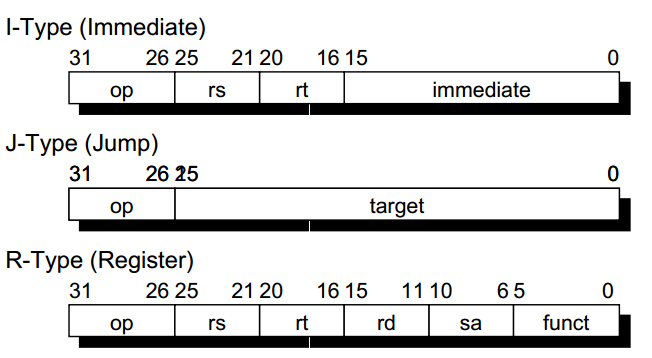
\includegraphics[width=0.8\textwidth]{./mips-formats}

\end{frame}

\begin{frame}[fragile]{Пример: код}
\begin{verbatim}
#define BITS(v, s, e) (v >> s) & (( 1 << (e-s+1)) - 1)
typedef struct decode {/* ... */} decode_t;
static inline int32_t sign_extend(uint32_t v, int width) 
    {/* ... */};
decode_t decode(uint32_t raw) {
    uint32_t op = BITS(raw, 26, 31);
    uint32_t rs = BITS(raw, 21, 25);
    uint32_t rt = BITS(raw, 16, 20);
    int32_t  imm = sign_extend(BITS(raw, 0, 15));
    int32_t  tgt = sign_extend(BITS(raw, 0, 25));
    /* ... */
    uint32_t funct = BITS(raw, 0, 5);
    return decode_t{op, rs, rt, imm, tgt, funct};
}
\end{verbatim}
\end{frame}

\begin{frame}{Более сложный пример: Intel IA-64 2.3}
\centering
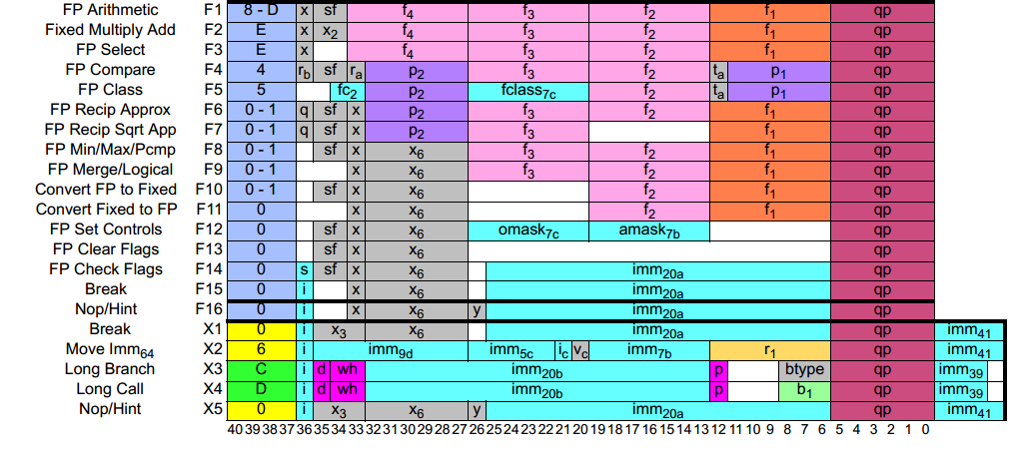
\includegraphics[width=0.95\textwidth]{./ia64-formats}

\tiny{Intel® Itanium® Architecture Software Developer’s Manual, p 3:296}

\end{frame}

\begin{frame}{Пример посложнее: Intel IA-32}
\centering
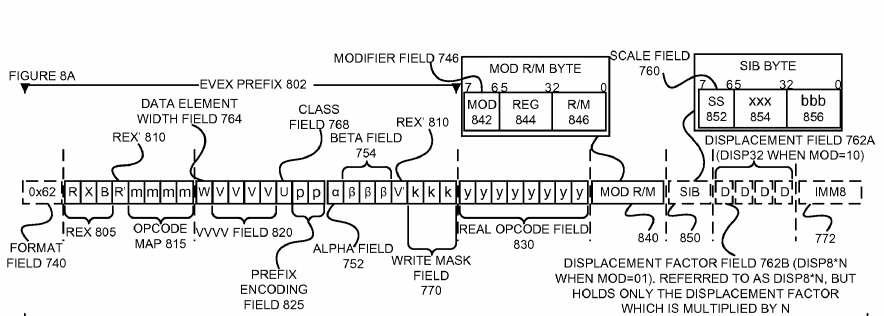
\includegraphics[width=0.95\textwidth]{./ia-32-evex}

\tiny{J.C.S. Adrian et al. Systems, Apparatuses, and Methods for Blending Two Source Operands into a Single Destination Using a Writemask. US Patent Application Publication. №~2012/0254588 A1}

\end{frame}

\begin{frame}{Что извлекать из машинного кода инструкции}
\centering
% This file allows to produce either a separate PDF/PNG image
% See standalone documentation to understand underlying magic

\documentclass[tikz,convert={density=150,size=600,outext=.png}]{standalone}
\usetikzlibrary{shapes, calc, arrows, fit, positioning, decorations, patterns, decorations.pathreplacing, chains, snakes}
\input{../setup-web-fonts}
\input{../setup-packages}
\graphicspath{{../pictures/}} % path to pictures, trailing slash is mandatory.

% The actual drawing follows
\begin{document}

\tikzstyle{FatArrow} = [thick, decoration={markings,mark=at position
        1 with {\arrow[semithick]{open triangle 60}}},
        double distance=1.4pt, shorten >= 5.5pt,
        preaction = {decorate},
        postaction = {draw,line width=1.4pt, white,shorten >= 4.5pt}]

\begin{tikzpicture}[font=\footnotesize, >=latex]
    \huge
    \node[rectangle, minimum height = 0.5cm] (mnemonic) {mnemonic,};
    \node[rectangle, right = 0.5cm of mnemonic.east, minimum height = 0.5cm] (src1) {src1,};
    \node[rectangle, right = 0.5cm of src1.east, minimum height = 0.5cm] (src2) {src2,};
    \node[rectangle, right = 0.5cm of src2.east, minimum height = 0.5cm] (dst1) {dst1};
    \node[draw, rectangle, right = 1.5cm of dst1.east, minimum height = 0.5cm] (dst2) {\textcolor{gray}{dst2}};

    \node[draw, fill=green, below = 2cm of mnemonic.south, minimum height = 0.5cm] (opcode) {Код операции};
    \node[draw, below = 2cm of src2.south, minimum height = 0.5cm] (regs) {Регистры, память, константы};
    \node[draw, fill=gray, align=center, below = 1.8cm of dst2.south, minimum height = 0.5cm] (flags) {Неявные операнды:\\ флаги, PC};

    \draw[FatArrow] (mnemonic) -- (opcode);
    \draw[FatArrow] (src1) -- ([xshift = 6.5mm] regs.north west);
    \draw[FatArrow] (src2) -- (regs);
    \draw[FatArrow] (dst1) -- ([xshift = -6.7mm] regs.north east);
    \draw[FatArrow] (dst2) -- (flags);

    \draw (mnemonic.south west) -- (dst1.south east) -- (dst1.north east) -- (mnemonic.north west) -- (mnemonic.south west);
\end{tikzpicture}

\end{document}
 % TODO convert to bitfields inlines

На выходе декодера: успех, неуспех, недостаточно данных.

\end{frame}


% \begin{frame}{Декодирование}
% Задача декодирования — перевод данных об инструкции из машинного представление
% во внутреннее (высокоуровневое) удобное для последующего анализа.

% \pause

% Вход: \texttt{\textcolor{red}{0x40} \textcolor{green}{0x05} \textcolor{blue}{0xab 0x12}}

% Результат:

% \texttt{instruction \{ \\
% ~~~~opcode = \textcolor{red}{ADDI}, num\_operands = 2, \\
% ~~~~\textcolor{green}{dst = \{type = OP\_REG, reg = R5\}}, \\
% ~~~~\textcolor{blue}{src = \{type = OP\_IMM, val = 0x12ab\}}, \\
% ~~~~disasm = "addi r5, 0x12ab", \\
% ~~~~addr = 0x1234 \\
% \}}
% \end{frame}

\begin{frame}{Декодирование}
Код декодера редко пишется вручную, чаще он генерируется по описанию.

\texttt{\textcolor{red}{A5} \textcolor{blue}{Y}\textcolor{green}{X} 0\textcolor{orange}{Z} 00} $\Rightarrow$ \textcolor{red}{MOD} \textcolor{green}{RX}, \textcolor{blue}{RY}, \textcolor{orange}{RZ}

В общем случае: классическаяя задача построения  синтаксического анализатора.

На практике: специализированные инструменты и языки.
\end{frame}

\begin{frame}{Декодирование: суровая реальность}
\begin{itemize}
\item Переменная длина инструкций. IA-32: от 8 до 120 бит. Сколько байт пытаться декодировать за один раз?
\item Зависимость смысла от префикса, режима работы процессора. Пример: 0x48
\item Полное несоответствие какому-либо здравому смыслу
\end{itemize}

\end{frame}

\begin{frame}{Дизассемблирование}
Дизассемблирование — перевод инструкций из машинного представление в понятный
человеку вид (мнемонику).\pause

(За)кодирование (encoding) — перевод инструкций из мнемонической записи в
машинный код.
\end{frame}

\section{Execute}

\begin{frame}{Исполнение}

Базовая единица — функция-эмулятор одной инструкции (service routine).

\bigskip

s.r. пишутся на языке высокого уровня — переносимость кода между хозяйскими
платформами, компиляторами.

\bigskip

Используются генераторы кода.

Пример: SimGen — из одного описания генерируются декодер, дизассемблер и s.r.

\end{frame}

\begin{frame}[fragile]{Пример: ADD}
\begin{verbatim}
void add32_rr(cpu_t *cpu, int src1, int src2, int dst) {
    cpu->regs[dst] = cpu->regs[src1] + cpu->regs[src2];
\end{verbatim}
\pause
\begin{verbatim}
    cpu->z_flag = cpu->regs[dst] == 0;
    cpu->n_flag = cpu->regs[dst] & (1 << 31);
    cpu->o_flag = cpu->regs[dst] < 
            MAX(cpu->regs[src1], cpu->regs[src2]);
    cpu->c_flag = calc_c_flag(cpu->regs[src1],
                              cpu->regs[src2]);
}
\end{verbatim}

\end{frame}

\begin{frame}{Пример посложнее}


\end{frame}

\section{Write Back}

\begin{frame}{Запись результата в память}

<<Обычная>> запись в память:

\pause

\begin{itemize}
    \item Невыровненные адрес,
    \item Граница страниц,
    \item Попытка изменить регион памяти доступный только для чтения,
    \item Часть результата может быть записана, а потом случится исключение.
\end{itemize}

\end{frame}

\section{Advance \texttt{PC}}

\begin{frame}{Продвижение \texttt{\$PC}}

\begin{itemize}
    \item Для большинства команд увеличение счетчика на длину обработанной инструкции. \\
    Ислючение: \texttt{REP MOVS}.
    \pause\bigskip
    \item Явное изменение \texttt{\$PC} — команды управления исполнением:
    \begin{itemize}
        \item (Un)conditional (In)direct Jump/Branch,
        \item Call/Return (subroutine).
    \end{itemize}
\end{itemize}

\end{frame}


\section{Исключения}

\begin{frame}[shrink=0.6]{Уточнённый цикл работы процессора}
\centering

\include{./../../simbook/metoda/drawings/interp-cycle-expanded-exception}

\end{frame}

\begin{frame}{Классификация}
Interruptions (термин из документации IA-64) — вмешательство, перерыв, приостановка
Exception — синхронное исключение, без повторения текущей инструкции
Fault — синхронное, с повторением текущей инструкции
Trap — синхронные, общий случай для некоторой инструкции
Interrupt — внешнее асинхронное прерывание
Abort — внешние асинхронное с отсутствием информации о точке возврата
\end{frame}


\section*{Конец}
% The final "thank you" frame 


\begin{frame}{На следующей лекции}
\end{frame}


\begin{frame}

{\huge{Спасибо за внимание!}\par}

\vfill

\tiny{\textit{Замечание}: все торговые марки и логотипы, использованные в данном материале, являются собственностью их владельцев. Представленная здесь точка зрения отражает личное мнение автора, не выступающего от лица какой-либо организации.}

\end{frame}

\end{document}
